The experiment shows that after only 10 days of exploration, the corporate could start to exploit good superarms, converging to the optimal one after about half a month.

This result is achieved because the combinatorial problem is solved in an exact way, thus increasing the execution time but lowering the additional regret. This is a reasonanble assumption as the corporate can run the algorithm over the night or in any time with low orders.
\\The approximation of the solution of the combinatorial problem would have saved just few minutes of computation but would have increased the regret of a non-trascurable amount of money, as a luxury brand cannot afford to sell products even with a sightly wrong price.
\\The cumulative regret when the algorithm learns both the conversion rate curves and the performance of the advertising subcampaigns is plotted as follows, along with its complementary reward chart that shows the reward at each time $t \in T$.
\\
\makebox[\textwidth][c]{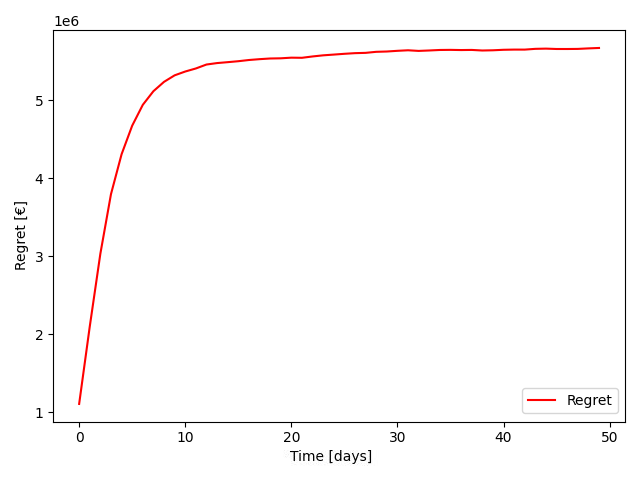
\includegraphics[width=0.9\textwidth]{../curves/results/bdgalloc_and_pricing_real_regret}}
\makebox[\textwidth][c]{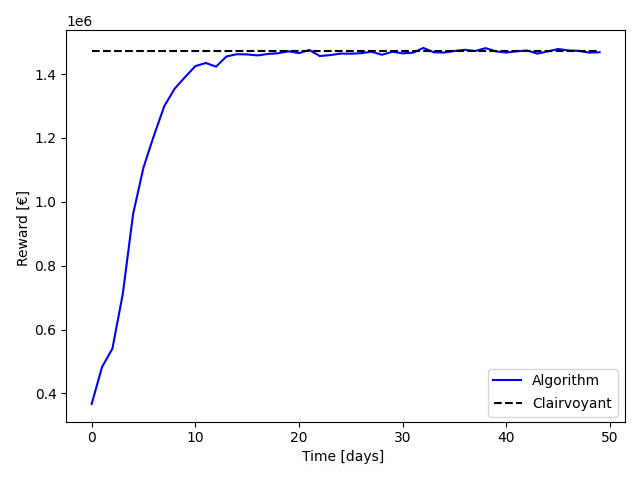
\includegraphics[width=0.9\textwidth]{../curves/results/bdgalloc_and_pricing_real_reward}}
